\section{Definitions}
\subsection{Tracklet}
\label{def:tracklet}
Yes you guessed it right, tracklet is basically a short track between 5 or 6 frames generally. Track generally refers to the entire trajectory of a unique object's (person) path. During training, we give short paths of different individuals referred to as tracklet. AFAIK, short paths are chosen because most tracking algorithms use a constant velocity linear motion model - and short tracks are usually straight lines and change is velocity is very small.

The term is very informal, as I couldn't find any literature about it as well when I was working on a tracking problem.

Reference: \href{https://stackoverflow.com/questions/55512548/whats-the-difference-between-track-and-tracklet-in-tracking}{What's the difference between track and tracklet in tracking?}

\subsection{Phases of the cell cycle}
\begin{figure}[!htb]
    \centering
    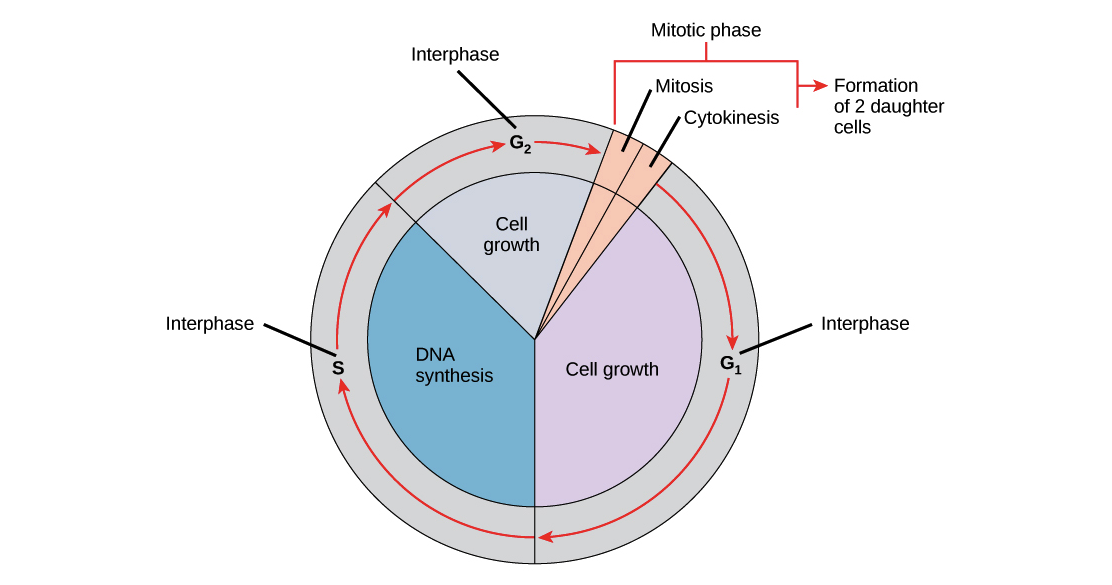
\includegraphics[width=\textwidth]{figures/cell_cycle.png}
    \caption{The cell cycle consists of interphase and the mitotic phase. During interphase, the cell grows and the nuclear DNA is duplicated. Interphase is followed by the mitotic phase. During the mitotic phase, the duplicated chromosomes are segregated and distributed into daughter nuclei. The cytoplasm is usually divided as well, resulting in two daughter cells.}
    \label{fig:cellcycle}
\end{figure}
Reference: \href{https://www.khanacademy.org/science/biology/cellular-molecular-biology/mitosis/a/cell-cycle-phases}{Phases of the cell cycle}, \href{http://cnx.org/contents/185cbf87-c72e-48f5-b51e-f14f21b5eabd@9.87:52/The-Cell-Cycle}{The Cell Cycle}
